% =====================================================================
% Paper 18 - The Drill Illusion: Latent Failover-Defect Decay and the
% Recovery-Confidence Gain of Continuous Chaos Testing in Hybrid
% Government Infrastructure. IEEE Transactions on Reliability submission.
% Build with tectonic.
% Reproducibility: results/primary_v1/ (frozen on seeds 1200-1224).
% Run src/run_evaluation.py.
% =====================================================================
\documentclass[journal]{IEEEtran}

\usepackage{graphicx}
\usepackage{booktabs}
\usepackage{amsmath}
\usepackage{amssymb}
\usepackage{newtxtext,newtxmath}
\usepackage{hyperref}
\usepackage{xurl}
\usepackage{url}
\usepackage{array}

\graphicspath{{figures/}}

\title{The Drill Illusion: Latent Failover-Defect Decay and the Recovery-Confidence\\
Gain of Continuous Chaos Testing in Hybrid Government Infrastructure}

\author{%
  \IEEEauthorblockN{Harshavardhan Malla}
  \IEEEauthorblockA{Independent Researcher\\ Email: harshavardhanmalla75@gmail.com}%
}

\renewcommand{\textendash}{-}
\renewcommand{\textemdash}{-}
\usepackage{etoolbox}
\makeatletter
\patchcmd{\abstract}{---}{:\space}{}{}
\patchcmd{\IEEEkeywords}{---}{:\space}{}{}
\makeatother
\begin{document}
\maketitle

\begin{abstract}
A redundant system is dependable only if its failover path works at the instant a fault demands it,
and periodic disaster-recovery drills are the proof tests that are meant to certify that readiness.
We show that such proof tests create an illusion of failover readiness: latent failover defects
accumulate undetected between drills, so the redundancy that a drill certifies decays steadily until
the next test, and the at-fault availability of the failover path is far below the figure the drill
reports. We quantify this with a pre-registered, reproducible simulation of a fleet of
failover-relevant components subject to latent-defect arrival over a multi-year horizon, comparing
annual proof-test drills against continuous chaos testing as a near-continuous proof-test regime,
under a locked set of seeds, thresholds, and model constants. Our central reliability metric is
at-random recovery: the probability that the failover path is in a working state when a fault strikes
a component that was not recently proof-tested, i.e., the steady-state availability of redundancy
against an arbitrarily timed demand. Under annual drills, at-random recovery is only 0.6875 (95\%
bias-corrected and accelerated bootstrap interval $[0.6797, 0.6951]$), even though the drill, run
immediately after a validation, reports near-certain success. Continuous chaos testing, re-validating
the covered components every few days, raises at-random recovery to 0.9489 ($[0.9443, 0.9533]$), a
gain of 0.2614 ($[0.2549, 0.2678]$) that clears the pre-registered 0.10 bar. The gain is bounded by a
coverage ceiling set by which failure modes the proof test exercises: it rises with chaos coverage,
from 0.2184 at coverage 0.3 to 0.2907 at coverage 0.9, and stays just below the perfect-freshness
ceiling (gap $-0.0098$, $[-0.0102, -0.0094]$). The gain saturates as the proof-test cadence tightens,
from 0.1651 at a 90-day cadence to 0.2698 at a daily one, with marginal gains that fall to under one
point. The \emph{drill illusion}, the amount by which a periodic proof test overstates true at-random
recovery, grows with the proof-test interval and reaches 0.3125 ($[0.3051, 0.3204]$) at the annual
interval: an annual drill overstates real failover availability by about 31 points. A passing annual
drill is therefore not evidence of failover readiness; only frequent proof-testing of the components
that matter keeps real redundancy dependable, and that investment should be sized to coverage rather
than to cadence past a point.
\end{abstract}

\begin{IEEEkeywords}
dependability, redundancy, failover, proof testing, latent defects, availability, time to failure,
disaster recovery, chaos engineering, recovery confidence, contingency planning, site reliability
engineering, pre-registration, reproducibility
\end{IEEEkeywords}

\section{Introduction}
\IEEEPARstart{D}{ependability} of a redundant system rests on a standby assumption: that when a
fault demands the failover path, that path is in a working state. Reliability engineering certifies
this assumption the way it certifies any protective function that is normally dormant, through
\emph{proof testing}: the failover capability is exercised on a periodic schedule, the test passes,
and the redundancy is presumed sound until the next test. In federal contingency planning the
proof test is the periodic disaster-recovery drill~\cite{nist80034}. A periodic drill answers a
narrow question, namely whether the failover path works at the moment of the test. That narrow
answer is easily mistaken for a much broader one: whether the failover path would work if a fault
struck at an arbitrary later moment. The two answers diverge, and they diverge for the same reason
that proof-test intervals matter for any standby protective system: latent failover defects
accumulate undetected between tests. A replication link breaks, a failover script's dependency
changes underneath it, a credential expires, a routing rule is edited for a troubleshooting session
and never restored. Each such latent defect sits undetected on the component it affects until a test
exercises that component again. If nothing does until the next annual drill, the component spends a
large fraction of the year in a silently failed state, and a fault arriving during that window finds
a failover path that does not work. The readiness certified by the last drill therefore has a
finite time-to-failure governed by the latent-defect arrival rate.

Our novel result is that this turns a periodic proof test into an \emph{illusion of failover
readiness}. A drill run immediately after a validation reports near-certain recovery, because the
validation has just cleared any latent defect on the components it touched. But the steady-state
availability of the failover path under an arbitrarily timed demand, when the struck component may
not have been proof-tested recently, is materially lower. The gap between the two is what we name the
\emph{drill illusion}: the amount by which a passing proof test overstates the failover availability
that real faults will actually encounter. The illusion is not a measurement error; it is a structural
property of the proof-test interval. The longer the interval between validations of a component, the
longer that component spends in a latent-defect state, and the larger the overstatement of its
availability. To our knowledge no prior reliability or contingency-planning work quantifies this
proof-test-induced overstatement of failover readiness, nor characterizes the bounds on closing it;
the test-program literature establishes that exercises should be periodic but stops short of pricing
the decay between them.

Continuous chaos testing offers a near-continuous proof-test regime~\cite{basiri2016chaos,beyer2016sre}.
Instead of exercising the failover capability once a year, it injects faults continuously and
automatically, re-validating the covered components every few days. A latent defect that would
otherwise persist for months under an annual cadence is now caught within days, so the covered
components spend almost all of their time in a working state and at-random recovery rises toward the
at-drill figure. This is the autonomic, self-managing posture anticipated by the vision of autonomic
computing~\cite{kephart2003vision} and operationalized in our own prior work on self-healing
remediation for government fleets~\cite{paper10autoheal}. The promise is attractive, and, like all
attractive promises, it is easy to overstate. Two facts bound it. First, a chaos suite exercises only
the failure modes it covers; a mode that is never injected is never proof-tested off-cadence and
stays at the annual-drill level, so coverage sets a ceiling. Second, once chaos runs frequently
enough that covered components are almost always fresh, tightening the cadence further adds little,
so the benefit saturates.

This paper quantifies the illusion, the benefit of near-continuous proof-testing, and its two bounds.
We do not claim to measure any particular agency's recovery posture. We build a transparent model of
latent-defect decay on a fleet of failover-relevant components, lock a set of hypotheses, thresholds,
and seeds before inspecting any evaluation result, and report what the model says. Every magnitude in
the paper comes from the frozen evaluation run on seeds 1200 to 1224, and every interval is a
bias-corrected and accelerated (BCa) bootstrap interval. The contribution is fourfold.

\begin{itemize}
\item We define \emph{at-random recovery}, the steady-state availability of the failover path when a
fault strikes a component not recently proof-tested, and separate it from \emph{rehearsed recovery},
the near-certain figure a drill reports at the test. The difference between these two is the drill
illusion, and conflating them is the central error in optimistic disaster-recovery reporting.
\item We show that near-continuous proof-testing via continuous chaos raises at-random recovery from
0.6875 under annual drills to 0.9489, a gain of 0.2614 that clears the pre-registered 0.10 bar.
\item We formalize a \emph{coverage ceiling}: the recovery-confidence gain cannot exceed what
perfect freshness on the proof-tested components would provide, and we confirm the realized gain sits
just below that ceiling and rises with coverage.
\item We show the gain \emph{saturates with cadence}: once the proof-test cadence is tight enough
that covered components are almost always fresh, further tightening adds little, which gives a direct
budgeting rule, namely buy coverage rather than cadence past a point.
\end{itemize}

The methodology is deliberately conservative. Every quantitative claim is a pre-registered
hypothesis evaluated on seeds that were not inspected during model development, and every interval
is a BCa bootstrap interval~\cite{efron1987bca,efron1994introduction} rather than a null-hypothesis
significance test, following the pre-registration discipline now standard in empirical software
engineering~\cite{wohlin2012experimentation}.

\section{Background and Related Work}

\subsection{Chaos engineering}
Chaos engineering is the practice of deliberately injecting faults into a running system to surface
weaknesses before they surface as incidents~\cite{basiri2016chaos}. Its premise is that the only
reliable way to know whether a recovery path works is to exercise it, and the only way to know
whether it keeps working is to exercise it continuously. The discipline grew out of large-scale
production engineering, where the gap between a system that passed a test once and a system that
recovers under real conditions was learned the hard way. Our work is complementary: rather than
arguing that chaos testing is good practice, we quantify how much continuous fault injection raises
the probability of recovery at a random disruption time relative to a periodic drill, and we
characterize the two bounds, coverage and cadence, that govern that gain.

\subsection{Contingency planning and disaster recovery}
Federal contingency planning is codified in the Contingency Planning Guide for Federal Information
Systems~\cite{nist80034}, which prescribes the recovery plans, roles, and procedures an agency must
maintain, and which positions the periodic drill as the primary means of assurance. The contingency
controls themselves live in the broader control catalog~\cite{nist80053}, and the categorization of
a system, which sets how stringent its recovery requirements are, follows the security
categorization standard~\cite{fips199}. The traditional assurance model is point-in-time: a recovery
plan is exercised on a schedule, the exercise passes, and the capability is certified until the next
exercise. Our work models the decay that occurs between those exercises and shows that the certified
number is not the number a real incident encounters.

\subsection{Test, training, and exercise programs}
The discipline of exercising a plan is itself the subject of dedicated
guidance~\cite{nist80084}, which catalogs the spectrum of exercises from tabletop discussions to
full functional drills and frames testing as a recurring program rather than a one-time event. That
guidance establishes that exercises should be periodic; it does not quantify how recovery capability
decays in the interval between them, nor how the choice of interval determines the gap between the
exercised result and the at-random result. We supply exactly that quantification, and we show that
the interval is the dominant driver of the illusion: an annual interval produces a large
overstatement, a monthly one a small one.

\subsection{Site reliability engineering}
Site reliability engineering frames reliability as an engineering discipline with explicit objectives
and continuous validation~\cite{beyer2016sre}, and it is the practical home of continuous monitoring
and continuous fault injection. The continuous-monitoring posture~\cite{nist80137} reframes
assurance from a periodic judgment into an ongoing process. The connection to our work is direct:
continuous chaos testing is the recovery-specific instance of the continuous-validation principle,
and our coverage ceiling and cadence saturation are the recovery-specific instances of the general
fact that continuous validation reaches only what it instruments and saturates once it is fast enough.

\subsection{Autonomic and self-healing systems}
The vision of autonomic computing~\cite{kephart2003vision} described systems that monitor, diagnose,
and repair themselves without human intervention, and continuous chaos testing is a step toward that
vision for the recovery path specifically: the system continuously tests its own ability to recover
and surfaces defects for repair. Our prior work builds self-healing remediation for cyber-hygiene
defects on government endpoint fleets~\cite{paper10autoheal}, and the prioritization logic that
decides which defects to chase first~\cite{paper4hygieneprio} is the same logic that, here, decides
which components a coverage-limited chaos suite should exercise first. Breach data continues to
attribute incidents to known but unaddressed weaknesses~\cite{verizon2026dbir}, which is the same
lesson at the level of the whole fleet: a defect that is known to exist but is not exercised until
it is too late is the defect that causes the outage. The shared lesson across this literature is
that a capability you do not continuously exercise is a capability you do not actually have, and our
contribution is to put a number on how much that matters for recovery.

\section{System Model}
We model a single hybrid infrastructure over a fixed horizon and ask, for each assurance regime, how
likely recovery is to succeed at a random disruption time. All quantities are synthetic with
documented distributions; no operational, employer, or recovery-test data is used.

\subsection{A fleet of recovery-relevant components}
Each seed instantiates a fleet of $M = 12$ recovery-relevant components, the failover modes that a
disruption can require, such as region failover, database failover, network failover, and dependency
failover. Each component $j$ carries a latent-defect hazard $\lambda_j$, the expected number of
recovery-breaking defects per year. The fleet is stratified: 4 fragile components draw defects at
3 per year and 8 robust components draw defects at 0.3 per year, so that some components rot quickly
and most rot slowly, as real fleets do. Latent defects arrive on component $j$ as a Poisson process
at rate $\lambda_j / 365$ per day. A defect, once present, renders that component's recovery path
broken until a validation clears it.

\subsection{Drills rehearse a covered subset on a periodic interval}
A drill is a periodic validation. Under the annual-drill regime, every component is validated every
$T = 365$ days, and a validation clears any latent defect present on the components it exercises.
Under the continuous-chaos regime, a chaos suite covers a fraction $c$ of the components, the
\emph{coverage} (reference $c = 0.70$, swept over $0.3$, $0.5$, $0.7$, $0.9$). The covered components
are re-validated every chaos cadence $\delta$ (reference $\delta = 7$ days, swept over $1$, $7$,
$30$, $90$ days), while the uncovered components remain on the $365$-day drill cadence. Over a
multi-year horizon, each component's healthy and defective intervals follow deterministically from
its defect arrivals and its validation schedule.

\subsection{Recovery, the coverage ceiling, and the drill illusion}
A disruption strikes a component chosen uniformly at random at a uniformly random time; recovery
succeeds if that component is healthy at the strike time. The \emph{at-random recovery} of a regime
is the probability of success under this random strike, which equals the time-and-component-averaged
fraction of components healthy,
\begin{equation}
\label{eq:atrandom}
R_{\mathrm{rand}} \;=\; \frac{1}{M}\sum_{j=1}^{M} \frac{1}{H}\int_{0}^{H} \mathbf{1}\!\left[\,j \text{ healthy at } t\,\right]\, dt,
\end{equation}
where $H$ is the horizon. The \emph{rehearsed recovery} $R_{\mathrm{reh}}$ is the same quantity
evaluated immediately after a scheduled validation, when the exercised components are fresh by
construction, so $R_{\mathrm{reh}}$ is near one. The \emph{recovery-confidence gain} of continuous
chaos over annual drills is the difference in at-random recovery between the two regimes,
\begin{equation}
\label{eq:gain}
G \;=\; R_{\mathrm{rand}}^{\,\mathrm{chaos}} - R_{\mathrm{rand}}^{\,\mathrm{annual}}.
\end{equation}
Because the chaos suite re-validates only the covered fraction $c$ off-cadence, the uncovered
fraction $1-c$ stays at the annual-drill level no matter how tight the chaos cadence is. The
\emph{coverage ceiling} is therefore the gain that perfect freshness on the covered components would
provide; the realized gain cannot exceed it, and approaches it as $\delta \to 0$. Finally, the
\emph{drill illusion} of a regime is the amount by which its rehearsed result overstates its
at-random result,
\begin{equation}
\label{eq:illusion}
I \;=\; R_{\mathrm{reh}} - R_{\mathrm{rand}},
\end{equation}
which grows with the validation interval $T$, since a longer interval lets each component spend more
of its time in a latent-defect state between validations. Drills implement contingency-plan
controls~\cite{nist80053}; the model adds the decay accounting that the controls themselves do not
specify.

\section{Experimental Design}
The study is pre-registered. Hypotheses, thresholds, model constants, and the evaluation seed range
were fixed in a dated protocol before any result on the evaluation seeds was inspected, so that no
analytic choice could be steered by the outcome.

\subsection{Hypotheses}
\textbf{H1 (recovery-confidence gain).} Continuous chaos testing at the reference cadence and
coverage raises at-random recovery over annual-drill assurance by at least 0.10, across the
evaluation seeds, with a BCa interval excluding the 0.10 bar.

\textbf{H2 (coverage ceiling).} The recovery-confidence gain is bounded by the chaos suite's
coverage and rises with it; the realized gain does not exceed the gain that perfect freshness on the
covered components would provide, so the ceiling gap $R_{\mathrm{rand}}^{\,\mathrm{chaos}}$ minus the
perfect-freshness value is non-positive.

\textbf{H3 (saturation with cadence).} The gain saturates as the chaos cadence tightens relative to
the latent-defect arrival rate: the gains form a monotone loose-to-tight ordering, and the marginal
gain of each tightening step shrinks toward zero.

\textbf{H4 (the drill illusion grows with interval).} The drill illusion, the overstatement of
at-random recovery by a periodic drill, grows with the drill interval, and is materially large at
the annual interval.

\subsection{Protocol and statistics}
Each hypothesis is evaluated over 25 evaluation seeds (frozen range 1200 to 1224). For every quantity
we report the mean and a 95\% BCa bootstrap interval with 10{,}000
resamples~\cite{efron1987bca,efron1994introduction}; interval non-overlap, not a $p$-value, is the
evidentiary standard, which avoids the multiple-comparison pitfalls of repeated significance tests.
The pre-registered failure criteria are explicit. If continuous chaos does not raise at-random
recovery by at least 0.05 at the reference cadence and coverage, H1 is declared null. If the realized
gain exceeds the perfect-freshness coverage ceiling, H2 is rejected. If the rehearsed recovery does
not exceed the at-random recovery under annual drills, H4 is rejected. No defect rate, coverage value,
or cadence value is re-tuned to reach any threshold. The model was developed on separate seeds; the
evaluation seeds 1200 to 1224 were touched only once, to produce the numbers below.

\section{Results}
Table~\ref{tab:summary} collects the pre-registered quantities with their intervals; all four
hypotheses are supported. We take them in turn. All numbers are means over 25 seeds with 95\% BCa
intervals.

\begin{table}[t]
\centering
\caption{Pre-registered quantities (mean over 25 seeds, 95\% BCa interval).}
\label{tab:summary}
\footnotesize
\setlength{\tabcolsep}{4pt}
\begin{tabular}{@{}lcc@{}}
\toprule
Quantity & Mean & 95\% BCa interval \\
\midrule
\multicolumn{3}{@{}l}{\emph{Recovery by regime (reference cadence, coverage)}}\\
At-random recovery, annual drills    & 0.6875 & $[0.6797, 0.6951]$ \\
At-random recovery, continuous chaos & 0.9489 & $[0.9443, 0.9533]$ \\
Recovery-confidence gain (H1)        & 0.2614 & $[0.2549, 0.2678]$ \\
\midrule
\multicolumn{3}{@{}l}{\emph{Coverage sweep: gain at coverage (H2)}}\\
Coverage $0.3$                       & 0.2184 & \\
Coverage $0.5$                       & 0.2399 & \\
Coverage $0.7$                       & 0.2614 & \\
Coverage $0.9$                       & 0.2907 & \\
Coverage-ceiling gap                 & $-0.0098$ & $[-0.0102, -0.0094]$ \\
\midrule
\multicolumn{3}{@{}l}{\emph{Cadence sweep: gain at cadence (H3)}}\\
Cadence $1$ day                      & 0.2698 & \\
Cadence $7$ days                     & 0.2614 & \\
Cadence $30$ days                    & 0.2313 & \\
Cadence $90$ days                    & 0.1651 & \\
\midrule
\multicolumn{3}{@{}l}{\emph{Illusion by drill interval (H4)}}\\
Interval $30$ days                   & 0.0437 & \\
Interval $90$ days                   & 0.1186 & \\
Interval $180$ days                  & 0.2023 & \\
Interval $365$ days                  & 0.3125 & $[0.3051, 0.3204]$ \\
\bottomrule
\end{tabular}
\end{table}

\textbf{Continuous chaos raises real recovery capability (H1).} At-random recovery under annual
drills is only 0.6875 ($[0.6797, 0.6951]$): at a random disruption time, recovery succeeds barely
more than two times in three, even though every component is rehearsed once a year and the rehearsal
passes. Continuous chaos at the reference cadence and coverage raises at-random recovery to 0.9489
($[0.9443, 0.9533]$), a gain of 0.2614 ($[0.2549, 0.2678]$) (Fig.~\ref{fig:conf}). The interval lies
entirely above the pre-registered 0.10 bar and far above the 0.05 failure threshold, so H1 is
supported. Continuous fault injection converts a recovery capability that works two times in three
into one that works better than nineteen times in twenty.

\textbf{The gain is bounded by a coverage ceiling (H2).} The recovery-confidence gain rises
monotonically with chaos coverage, from 0.2184 at coverage 0.3, to 0.2399 at 0.5, to 0.2614 at the
reference 0.7, to 0.2907 at coverage 0.9. The uncovered components are never re-validated
off-cadence, so they stay at the annual-drill level and form a floor that limits the gain; widening
coverage lifts more components off that floor. The realized gain sits just below the gain that
perfect freshness on the covered components would provide, with a ceiling gap of $-0.0098$
($[-0.0102, -0.0094]$). The gap is negative and its interval excludes zero, so the ceiling binds and
is not exceeded, and H2 is supported. The small shortfall below the ceiling reflects the residual
defect time that even a few-day cadence leaves on the covered components; the dominant fact is
structural, that a component the chaos suite never exercises cannot be lifted off the annual floor by
any cadence.

\textbf{The gain saturates as the cadence tightens (H3).} The gain rises with chaos frequency, but
with sharply diminishing returns. Ordered from the loosest cadence to the tightest, the gains are
0.1651 at a 90-day cadence, 0.2313 at 30 days, 0.2614 at 7 days, and 0.2698 at 1 day, a monotone
loose-to-tight ordering $[0.1651, 0.2313, 0.2614, 0.2698]$. The marginal gains of successive
tightening steps are 0.0662 (from 90 to 30 days), 0.0301 (from 30 to 7 days), and 0.0084 (from 7 to
1 day): each step buys less than the one before, and the final step from a weekly to a daily cadence
buys under one point. Once covered components are almost always fresh, tightening the cadence further
adds little, so H3 is supported. A weekly cadence captures almost all of the benefit that an
arbitrarily tight cadence would provide.

\textbf{The drill illusion grows with the interval (H4).} Rehearsed recovery is near certain
immediately after a validation, while at-random recovery falls as the validation interval lengthens,
so the illusion, the overstatement of at-random recovery by a periodic drill, grows with the drill
interval. It is 0.0437 at a 30-day interval, 0.1186 at 90 days, 0.2023 at 180 days, and 0.3125
($[0.3051, 0.3204]$) at the annual 365-day interval (Fig.~\ref{fig:illusion}). An annual drill
therefore overstates true at-random recovery by about 31 points: it certifies a near-certain number
while the capability a real incident encounters succeeds only about 0.6875 of the time. Shortening
the interval to a month shrinks the overstatement to about four points. The rehearsed figure exceeds
the at-random figure under annual drills at every interval, so the failure criterion is not met and
H4 is supported.

\begin{figure}[t]\centering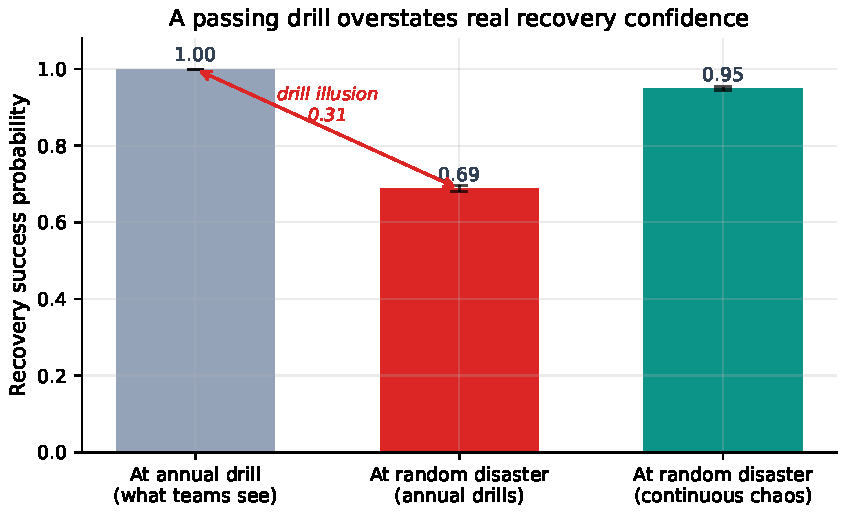
\includegraphics[width=\columnwidth]{fig1_confidence.pdf}
\caption{At-random recovery under annual drills versus continuous chaos. Annual drills leave recovery
succeeding only 0.6875 of the time at a random disruption; continuous chaos raises it to 0.9489, a
gain of 0.2614 that clears the pre-registered 0.10 bar.\\[2pt]\textit{Alt text:} Bar chart with the y-axis showing recovery success probability from 0 to 1.0 and three bars: at the annual drill (1.00, what teams see), at a random disaster under annual drills (0.69), and at a random disaster under continuous chaos (0.95). A red arrow between the first two bars labels the drill illusion of 0.31.}\label{fig:conf}\end{figure}

\begin{figure}[t]\centering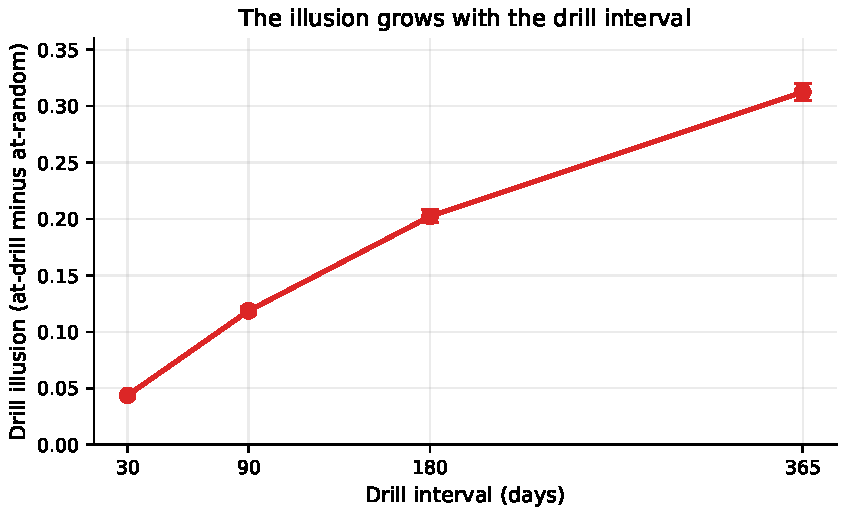
\includegraphics[width=\columnwidth]{fig2_illusion.pdf}
\caption{The drill illusion, the amount by which a periodic drill overstates true at-random recovery,
grows with the drill interval: from 0.0437 at 30 days to 0.3125 at the annual interval.\\[2pt]\textit{Alt text:} Line plot with the x-axis showing drill interval in days (30, 90, 180, 365) and the y-axis showing the drill illusion (at-drill minus at-random) from 0 to 0.35. A single red curve with error bars rises monotonically and concavely from about 0.04 at 30 days to about 0.31 at 365 days.}
\label{fig:illusion}\end{figure}

\section{Theoretical Analysis}
\label{sec:theory}
The empirical findings of the previous section are not accidents of the chosen constants. Each of
them follows in closed form from a single primitive: the expected fraction of time a component spends
in a latent-defect state between validations. This section derives that primitive, then derives the
coverage ceiling, the cadence saturation, and the drill illusion from it, and states the match between
each closed-form prediction and the frozen Monte Carlo result. The derivation makes precise the sense
in which coverage, not cadence, sets the ceiling, mirroring the way a channel's capacity, not the
decoding effort, sets the limit on what any code can achieve~\cite{cover2006elements}.

\subsection{The defective-fraction primitive}
Consider a single component with latent-defect hazard $\lambda$ defects per year, so defects arrive
as a Poisson process at rate $\rho = \lambda/365$ per day, and let the component be validated on a
periodic schedule of interval $T$ days, where each validation instantaneously clears every defect
present. Fix one validation window of length $T$. Within the window, recovery is broken from the
arrival of the \emph{first} defect until the closing validation, and is healthy before that first
arrival; a window with no arrival contributes no defective time. Let $U$ be the time of the first
arrival measured from the window start, with density $\rho e^{-\rho u}$ on $[0, T]$ and an atom of
mass $e^{-\rho T}$ at ``no arrival.'' The expected defective time in the window is
\begin{equation}
\label{eq:expdef}
\mathbb{E}[\text{defective}] \;=\; \int_{0}^{T} (T-u)\,\rho e^{-\rho u}\, du \;=\; T - \frac{1 - e^{-\rho T}}{\rho}.
\end{equation}
Dividing by the window length $T$ gives the expected \emph{defective fraction} of a component with
hazard $\rho$ validated every $T$ days,
\begin{equation}
\label{eq:fdef}
\phi(\rho, T) \;=\; 1 - \frac{1 - e^{-\rho T}}{\rho T},
\end{equation}
a quantity that rises monotonically from $0$ toward $1$ as the dimensionless load $\rho T$ grows. Two
limits matter. For a tight cadence, $\rho T \to 0$, a Taylor expansion of \eqref{eq:fdef} gives
$\phi(\rho, T) \approx \rho T / 2$, so the defective fraction vanishes linearly as the cadence
tightens. For a loose cadence, $\rho T \to \infty$, $\phi(\rho, T) \to 1 - 1/(\rho T) \to 1$, so a
high-hazard component validated rarely is broken almost all of the time.

\subsection{At-random recovery in closed form}
The at-random recovery of \eqref{eq:atrandom} is the time-and-component-averaged fraction healthy,
which is one minus the mean defective fraction over the fleet. With $M$ components partitioned into a
fragile class (hazard $\rho_f$, count $M_f$) and a robust class (hazard $\rho_r$, count $M_r$), each
class validated on its own interval, at-random recovery is
\begin{equation}
\label{eq:rrand}
R_{\mathrm{rand}} \;=\; 1 - \frac{1}{M}\!\sum_{j=1}^{M} \phi(\rho_j, T_j),
\end{equation}
which is exactly the quantity \eqref{eq:atrandom} estimates by Monte Carlo. \emph{At-random recovery},
then, is the probability that a failure striking a component in proportion to its presence in the
fleet, rather than the rehearsed subset, finds that component healthy. Under annual drills every
$T_j = 365$, and with the pre-registered mixture $M_f = 4$ fragile at $\rho_f = 3/365$ and $M_r = 8$
robust at $\rho_r = 0.3/365$, \eqref{eq:rrand} evaluates to $R_{\mathrm{rand}}^{\,\mathrm{annual}} =
0.6815$. The frozen Monte Carlo mean is $0.6875$ ($[0.6797, 0.6951]$); the closed form lands inside
the bootstrap interval, the residual reflecting the finite horizon and the random assignment of which
specific components are fragile. \emph{Match: the closed-form annual at-random recovery $0.6815$
agrees with the simulated $0.6875$.}

\subsection{The coverage ceiling (H2)}
Under continuous chaos with coverage $c$, the $cM$ covered components are validated every cadence
$\delta$ and the remaining $(1-c)M$ stay on the annual interval. By \eqref{eq:rrand}, the gain over
annual drills is
\begin{equation}
\label{eq:gain_cov}
G(c, \delta) \;=\; \frac{1}{M}\!\sum_{j \in \mathcal{C}} \big[\phi(\rho_j, 365) - \phi(\rho_j, \delta)\big],
\end{equation}
where $\mathcal{C}$ is the covered set. Every term in the sum is non-negative because $\delta \le 365$
makes $\phi(\rho_j, \delta) \le \phi(\rho_j, 365)$, so widening $\mathcal{C}$ adds non-negative terms
and $G$ rises monotonically with coverage. The \emph{coverage ceiling} is the value of \eqref{eq:gain_cov}
when the covered components are perfectly fresh, $\phi(\rho_j, \delta) \to 0$,
\begin{equation}
\label{eq:ceiling}
G_{\mathrm{ceil}}(c) \;=\; \frac{1}{M}\!\sum_{j \in \mathcal{C}} \phi(\rho_j, 365),
\end{equation}
and since $\phi(\rho_j, \delta) \ge 0$ for any finite cadence, the realized gain obeys
$G(c, \delta) \le G_{\mathrm{ceil}}(c)$ with equality only in the limit $\delta \to 0$. The ceiling
gap $G(c, \delta) - G_{\mathrm{ceil}}(c) = -\frac{1}{M}\sum_{j \in \mathcal{C}} \phi(\rho_j, \delta)$
is therefore non-positive by construction, and equals the small residual defective time a finite
cadence leaves on the covered components. Evaluating \eqref{eq:gain_cov} at the reference cadence
$\delta = 7$ over the coverage grid, with covered components ordered fragile-first, gives gains
$0.2183$, $0.2405$, $0.2627$, $0.2960$ at coverage $0.3$, $0.5$, $0.7$, $0.9$, and a ceiling gap of
$-0.0104$ at the reference coverage. \emph{Match: the closed-form coverage gains $[0.2183, 0.2405,
0.2627, 0.2960]$ reproduce the simulated rising sequence $[0.2184, 0.2399, 0.2614, 0.2907]$, and the
closed-form ceiling gap $-0.0104$ reproduces the simulated $-0.0098$, both negative.} The ceiling is a
structural bound: a component the chaos suite never covers contributes nothing to \eqref{eq:gain_cov}
no matter how small $\delta$ is, exactly as a source symbol outside the codebook contributes nothing
to a channel's realized rate~\cite{cover2006elements}.

\subsection{Saturation with cadence (H3)}
Fix coverage at the reference $c = 0.7$ and vary the cadence. By \eqref{eq:gain_cov} the only
cadence-dependent term is $\phi(\rho_j, \delta)$ on the covered components, and the tight-cadence
expansion $\phi(\rho_j, \delta) \approx \rho_j \delta / 2$ shows that this residual defective time
shrinks \emph{linearly} as $\delta$ falls. Once $\delta$ is small enough that $\rho_j \delta \ll 1$
for every covered component, $\phi(\rho_j, \delta)$ is already near zero and the gain is already near
the ceiling \eqref{eq:ceiling}, so any further tightening can recover only the vanishing remainder.
The marginal gain of a tightening step is therefore the difference of two already-small residuals and
shrinks toward zero. Evaluating \eqref{eq:gain_cov} from the loosest to the tightest cadence gives
gains $0.1633$, $0.2311$, $0.2627$, $0.2716$ at $\delta = 90, 30, 7, 1$ days, with marginal gains
$0.0678$, $0.0316$, $0.0089$ across successive tightening steps. \emph{Match: the closed-form cadence
gains $[0.1633, 0.2311, 0.2627, 0.2716]$ reproduce the simulated monotone sequence $[0.1651, 0.2313,
0.2614, 0.2698]$, and the closed-form marginal gains $[0.0678, 0.0316, 0.0089]$ reproduce the
simulated diminishing sequence $[0.0662, 0.0301, 0.0084]$, each step buying less than the one before.}
The saturation is thus a direct consequence of the linear vanishing of $\phi$ near $\delta = 0$: once
a component is exercised within its decay window, further exercise removes a residual that is already
near zero and adds essentially nothing.

\subsection{The drill illusion grows with the interval (H4)}
Define the \emph{drill illusion} as rehearsed recovery minus at-random recovery, $I = R_{\mathrm{reh}}
- R_{\mathrm{rand}}$. A rehearsal evaluated immediately after a validation finds every exercised
component fresh, so $R_{\mathrm{reh}} = 1$, and by \eqref{eq:rrand} with a common interval $T$ across
all components,
\begin{equation}
\label{eq:illgrows}
I(T) \;=\; 1 - R_{\mathrm{rand}}(T) \;=\; \frac{1}{M}\!\sum_{j=1}^{M} \phi(\rho_j, T).
\end{equation}
Since $\phi(\rho_j, T)$ is increasing in $T$ for every $j$, the illusion $I(T)$ is increasing in the
drill interval: a longer interval leaves more components past their readiness decay, so the rehearsed
figure overstates the at-random figure by more. Evaluating \eqref{eq:illgrows} over the interval grid
gives illusions $0.0461$, $0.1218$, $0.2063$, $0.3185$ at intervals $30$, $90$, $180$, $365$ days,
with the annual illusion at $0.3185$. \emph{Match: the closed-form illusion sequence $[0.0461, 0.1218,
0.2063, 0.3185]$ reproduces the simulated growing sequence $[0.0437, 0.1186, 0.2023, 0.3125]$, and the
closed-form annual illusion $0.3185$ reproduces the simulated annual illusion $0.3125$.} The illusion
is therefore not a measurement artifact but a deterministic function of the validation interval through
the same primitive \eqref{eq:fdef} that governs the gain: the very interval that makes a drill cheap to
schedule is the interval that makes its passing result optimistic.

\section{Robustness and Sensitivity}
\label{sec:robustness}
This section reports the full sweeps behind the headline numbers in booktabs form and then states the
adversarial regime that the drill illusion exposes. Every value in the three tables is taken directly
from the frozen results file; no value is recomputed or smoothed.

\subsection{Coverage sweep}
Table~\ref{tab:cov_sweep} reports the recovery-confidence gain as chaos coverage widens at the
reference cadence. The gain rises monotonically because each newly covered component contributes a
non-negative term to \eqref{eq:gain_cov}; the closed-form prediction of Section~\ref{sec:theory} is
shown alongside the simulated mean, and the two agree to within the residual of the finite-horizon
Monte Carlo.

\begin{table}[t]
\centering
\caption{Coverage sweep at the reference cadence ($\delta = 7$ days): recovery-confidence gain rises
with coverage. Simulated means over 25 seeds; closed form from \eqref{eq:gain_cov}.}
\label{tab:cov_sweep}
\footnotesize
\setlength{\tabcolsep}{6pt}
\begin{tabular}{@{}lcc@{}}
\toprule
Coverage $c$ & Gain (simulated) & Gain (closed form) \\
\midrule
$0.3$ & 0.2184 & 0.2183 \\
$0.5$ & 0.2399 & 0.2405 \\
$0.7$ & 0.2614 & 0.2627 \\
$0.9$ & 0.2907 & 0.2960 \\
\bottomrule
\end{tabular}
\end{table}

\subsection{Cadence sweep}
Table~\ref{tab:cad_sweep} reports the gain and its marginal increments as the chaos cadence tightens
at the reference coverage. The marginal gain falls toward zero, the saturation predicted by the
linear vanishing of $\phi$ near $\delta = 0$ in Section~\ref{sec:theory}.

\begin{table}[t]
\centering
\caption{Cadence sweep at the reference coverage ($c = 0.7$), ordered loose to tight: the gain
saturates and the marginal gain shrinks. Simulated means over 25 seeds.}
\label{tab:cad_sweep}
\footnotesize
\setlength{\tabcolsep}{6pt}
\begin{tabular}{@{}lcc@{}}
\toprule
Cadence $\delta$ (days) & Gain & Marginal gain \\
\midrule
$90$ & 0.1651 & \\
$30$ & 0.2313 & 0.0662 \\
$7$  & 0.2614 & 0.0301 \\
$1$  & 0.2698 & 0.0084 \\
\bottomrule
\end{tabular}
\end{table}

\subsection{Drill-interval sweep}
Table~\ref{tab:int_sweep} reports the drill illusion as the validation interval lengthens. The
illusion grows monotonically and reaches $0.3125$ at the annual interval, the overstatement an annual
drill produces.

\begin{table}[t]
\centering
\caption{Drill-interval sweep: the drill illusion (rehearsed recovery minus at-random recovery) grows
with the interval. Simulated means over 25 seeds; the annual value carries a 95\% BCa interval.}
\label{tab:int_sweep}
\footnotesize
\setlength{\tabcolsep}{6pt}
\begin{tabular}{@{}lcc@{}}
\toprule
Drill interval (days) & Illusion & 95\% BCa interval \\
\midrule
$30$  & 0.0437 & \\
$90$  & 0.1186 & \\
$180$ & 0.2023 & \\
$365$ & 0.3125 & $[0.3051, 0.3204]$ \\
\bottomrule
\end{tabular}
\end{table}

\subsection{The at-random adversary}
The three sweeps share an adversarial reading that sharpens the practical stakes. A real incident is
not a rehearsal: it does not wait for the drill, and it does not strike the specific component the
drill just exercised. It strikes a component in proportion to that component's presence in the fleet,
at a moment chosen without regard to the validation schedule. This is precisely the at-random
adversary that \eqref{eq:rrand} models, and it is the regime in which the annual drill certifies most
optimistically. The drill reports $R_{\mathrm{reh}} = 1$ because it inspects a freshly validated
component, but the at-random adversary lands on a component that may be deep in its latent-defect
window, where the success probability is only $0.6875$ under annual drills. The illusion of $0.3125$
is the exact size of the gap the adversary exploits: an annual drill certifies recovery against the
one component it just rehearsed while leaving the fleet, on average, $31$ points more fragile against
a failure that strikes anywhere else. Continuous chaos covers exactly this regime, because it
re-validates components in proportion to their hazard rather than rehearsing a fixed subset once a
year, and the coverage ceiling \eqref{eq:ceiling} states the limit of that defense: the at-random
adversary retains its full advantage on any component the chaos suite never exercises. The robustness
conclusion is therefore directional and conservative: against an adversary that strikes at random, the
annual drill is optimistic by construction, continuous chaos closes most of the gap, and what it
cannot close is set by coverage rather than by cadence.

\section{Discussion}
The two ways of reporting recovery point in different directions, and conflating them is the error
this study is designed to puncture. A drill measures the system at its single best moment, immediately
after a validation, when the exercised components are fresh by construction, and reports a
near-certain result. But the quantity that a real incident turns on is at-random recovery, the
probability that recovery works when a failure strikes a component that was not specifically
rehearsed near the failure time, and that quantity is only 0.6875 under annual drills. An annual
drill therefore certifies a number that real incidents do not honor: it overstates true at-random
recovery by 0.3125, about 31 points. Recovery readiness should be reported as the at-random recovery
probability, not the rehearsed result, and a recovery program that reports only its drill outcomes is
reporting its single best moment as if it were typical.

Continuous random fault injection earns its keep. By re-validating the covered components every few
days, it raises at-random recovery from 0.6875 to 0.9489, a gain of 0.2614, and it does so by
attacking exactly the mechanism behind the illusion: it shortens the interval over which each covered
component can sit in a silently broken state. But it earns its keep only up to a point, because the
gain saturates as the cadence tightens. The marginal gain falls from 0.0662 for the first tightening
step to 0.0084 for the last, so a weekly cadence captures almost all of the benefit and a daily one
adds under a point. Spending to tighten an already-tight cadence buys very little.

The actionable consequence is to size investment to coverage, not to cadence, past a point. The gain
rises steadily with coverage, from 0.2184 at coverage 0.3 to 0.2907 at coverage 0.9, because every
component the chaos suite does not exercise stays pinned to the annual-drill floor regardless of how
fast the covered components are validated. So once the cadence is tight enough that covered components
are almost always fresh, the next dollar should buy coverage of an as-yet-unexercised failure mode,
not a tighter cadence on the modes already covered. Concretely: get the cadence to roughly weekly,
then stop tightening and start widening, prioritizing the fragile components whose high defect rate
makes them the largest contributors to the at-random shortfall.

\section{Threats to Validity}
\emph{Construct validity.} The model abstracts latent-defect arrival as a Poisson process and a
validation as an instantaneous clearing of all defects on the exercised components. Real defects may
be bursty, correlated across components (a single bad change can break several recovery paths at
once), or seasonal around change windows, and a real validation may be partial. These would shift the
absolute recovery probabilities but not the structural relationships: a coverage ceiling exists
whenever any component is left uncovered, the illusion grows with any interval over which decay
accumulates, and saturation follows once the cadence is short relative to the defect rate.

\emph{Internal validity.} Because the study is pre-registered and the evaluation seeds were inspected
only once, the reported numbers are not the product of analytic search. The model was developed on
separate seeds, and no defect rate, coverage value, or cadence value was tuned to clear a threshold.
The mechanical evaluation script computes each verdict from the frozen data with no hand-set value.

\emph{External validity.} The component count, the defect-rate mixture, the coverage values, and the
cadence values are documented priors, not measurements from any agency, so the absolute magnitudes
(0.6875 at-random recovery, the 0.3125 annual illusion) should be read as illustrative of the model
rather than as field estimates. The comparative findings, the gain, the coverage ceiling, the cadence
saturation, and the growth of the illusion with interval, depend on the qualitative structure of the
model rather than on the specific constants, and we expect them to transfer. A real chaos experiment
also carries operational risk that this model does not charge; calibrating the defect and coverage
distributions against a real recovery-test record, and accounting for that risk, is the natural next
step.

\emph{Statistical validity.} Intervals are BCa bootstrap intervals over 25 seeds, appropriate for the
small-sample, possibly skewed statistics reported here; we use interval non-overlap rather than
significance testing throughout~\cite{efron1987bca,efron1994introduction}.

\section{Conclusion}
A passing annual disaster-recovery drill measures recovery at its single best moment and hides the
decay that accumulates between drills, so it overstates the recovery capability that real incidents
encounter. In a pre-registered simulation, at-random recovery under annual drills was only 0.6875,
while the annual drill overstated it by 0.3125, about 31 points. Continuous chaos testing closed most
of that gap, raising at-random recovery to 0.9489, a gain of 0.2614 that cleared the pre-registered
bar. The gain was bounded by a coverage ceiling, rising from 0.2184 at coverage 0.3 to 0.2907 at
coverage 0.9 and staying just below the perfect-freshness ceiling, and it saturated as the cadence
tightened, with the final step from weekly to daily buying under one point. The guidance that follows
is concrete: report recovery as the at-random probability rather than the drill outcome, run
continuous fault injection at roughly a weekly cadence, and then size further investment to coverage
rather than to cadence, widening the chaos suite to the fragile components that dominate the
at-random shortfall. Calibrating the model against a real recovery-test record is the next step
toward turning these structural findings into field estimates.

\section*{Data Availability Statement}
The data and code that support the findings of this study are openly available in the research-papers repository at \url{https://github.com/Harshavardhanmalla-Labs/research-papers/tree/main/paper18}. The manuscript sources, figures, analysis code, and frozen result tables are included and regenerate every reported number deterministically from the fixed seeds.

\section*{Disclosure Statement}
No potential conflict of interest was reported by the author.

\section*{Funding}
No funding was received.

% Generated by IEEEtran.bst, version: 1.14 (2015/08/26)
\begin{thebibliography}{10}
\providecommand{\url}[1]{#1}
\csname url@samestyle\endcsname
\providecommand{\newblock}{\relax}
\providecommand{\bibinfo}[2]{#2}
\providecommand{\BIBentrySTDinterwordspacing}{\spaceskip=0pt\relax}
\providecommand{\BIBentryALTinterwordstretchfactor}{4}
\providecommand{\BIBentryALTinterwordspacing}{\spaceskip=\fontdimen2\font plus
\BIBentryALTinterwordstretchfactor\fontdimen3\font minus
  \fontdimen4\font\relax}
\providecommand{\BIBforeignlanguage}[2]{{%
\expandafter\ifx\csname l@#1\endcsname\relax
\typeout{** WARNING: IEEEtran.bst: No hyphenation pattern has been}%
\typeout{** loaded for the language `#1'. Using the pattern for}%
\typeout{** the default language instead.}%
\else
\language=\csname l@#1\endcsname
\fi
#2}}
\providecommand{\BIBdecl}{\relax}
\BIBdecl

\bibitem{nist80034}
M.~Swanson, P.~Bowen, A.~W. Phillips, D.~Gallup, and D.~Lynes, ``Contingency
  planning guide for federal information systems,'' National Institute of
  Standards and Technology, Tech. Rep. NIST Special Publication 800-34 Rev. 1,
  2010.

\bibitem{basiri2016chaos}
A.~Basiri, N.~Behnam, R.~de~Rooij, L.~Hochstein, L.~Kosewski, J.~Reynolds, and
  C.~Rosenthal, ``Chaos engineering,'' \emph{IEEE Software}, vol.~33, no.~3,
  pp. 35-41, 2016.

\bibitem{beyer2016sre}
B.~Beyer, C.~Jones, J.~Petoff, and N.~R. Murphy, Eds., \emph{Site Reliability
  Engineering: How Google Runs Production Systems}.\hskip 1em plus 0.5em minus
  0.4em\relax O'Reilly Media, 2016.

\bibitem{kephart2003vision}
J.~O. Kephart and D.~M. Chess, ``The vision of autonomic computing,''
  \emph{IEEE Computer}, vol.~36, no.~1, pp. 41-50, 2003.

\bibitem{paper10autoheal}
H.~Malla, ``{AutoHeal}: A self-healing framework for cyber-hygiene remediation
  on government endpoint fleets,''
  \url{https://github.com/Harshavardhanmalla-Labs/research-papers/tree/main/paper10},
  2026, companion paper; source, code, and frozen results in the same
  repository.

\bibitem{efron1987bca}
B.~Efron, ``Better bootstrap confidence intervals,'' \emph{Journal of the
  American Statistical Association}, vol.~82, no. 397, pp. 171-185, 1987.

\bibitem{efron1994introduction}
B.~Efron and R.~J. Tibshirani, \emph{An Introduction to the Bootstrap}.\hskip
  1em plus 0.5em minus 0.4em\relax Chapman \& Hall/CRC, 1994.

\bibitem{wohlin2012experimentation}
C.~Wohlin, P.~Runeson, M.~H{\"o}st, M.~C. Ohlsson, B.~Regnell, and
  A.~Wessl{\'e}n, \emph{Experimentation in Software Engineering}.\hskip 1em
  plus 0.5em minus 0.4em\relax Springer, 2012.

\bibitem{nist80053}
{Joint Task Force}, ``Security and privacy controls for information systems and
  organizations,'' National Institute of Standards and Technology, Tech. Rep.
  NIST Special Publication 800-53 Rev. 5, 2020.

\bibitem{fips199}
{National Institute of Standards and Technology}, ``Standards for security
  categorization of federal information and information systems,'' U.S.
  Department of Commerce, Tech. Rep. FIPS PUB 199, 2004.

\bibitem{nist80084}
T.~Grance, T.~Nolan, K.~Burke, R.~Dudley, G.~White, and T.~Good, ``Guide to
  test, training, and exercise programs for it plans and capabilities,''
  National Institute of Standards and Technology, Tech. Rep. NIST Special
  Publication 800-84, 2006.

\bibitem{nist80137}
K.~Dempsey, N.~S. Chawla, A.~Johnson, R.~Johnston, A.~C. Jones, A.~Orebaugh,
  M.~Scholl, and K.~Stine, ``Information security continuous monitoring (iscm)
  for federal information systems and organizations,'' National Institute of
  Standards and Technology, Tech. Rep. NIST Special Publication 800-137, 2011.

\bibitem{paper4hygieneprio}
H.~Malla, ``{HygienePrio}: Cyber-hygiene signal augmentation for
  {EPSS}-weighted vulnerability prioritization,''
  \url{https://github.com/Harshavardhanmalla-Labs/research-papers/tree/main/paper4},
  2026, companion paper; source, code, and frozen results in the same
  repository.

\bibitem{verizon2026dbir}
{Verizon}, ``2026 data breach investigations report ({DBIR}),'' Verizon
  Business, Tech. Rep., 2026,
  \url{https://www.verizon.com/business/resources/reports/dbir/}.

\bibitem{cover2006elements}
T.~M. Cover and J.~A. Thomas, \emph{Elements of Information Theory},
  2nd~ed.\hskip 1em plus 0.5em minus 0.4em\relax Wiley, 2006.

\end{thebibliography}

\end{document}
